\documentclass[tikz,border=10pt]{standalone}
\usepackage{amsmath}
% Scale: s = 0.01 cm per px (longest side ~8 cm, per STYLE METRICS)
\begin{document}
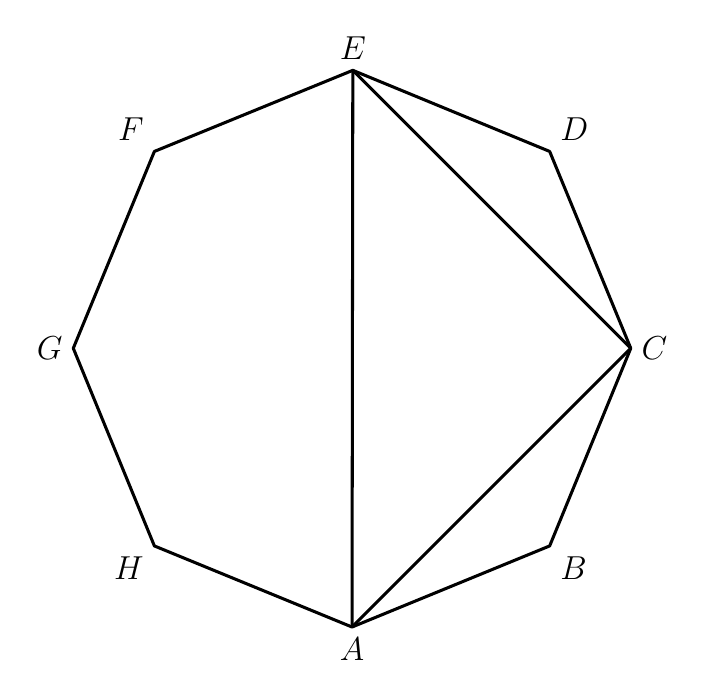
\begin{tikzpicture}[line join=round, line width=1.1pt]
  % Vertices (x=(px-456.5)*0.01, y=(452-py)*0.01)
  \coordinate (A) at (0.00,-3.54);
  \coordinate (B) at (2.51,-2.51);
  \coordinate (C) at (3.54,0.00);
  \coordinate (D) at (2.51,2.50);
  \coordinate (E) at (0.01,3.53);
  \coordinate (F) at (-2.51,2.50);
  \coordinate (G) at (-3.54,0.00);
  \coordinate (H) at (-2.51,-2.51);

  % Octagon edges
  \draw (A) -- (B) -- (C) -- (D) -- (E) -- (F) -- (G) -- (H) -- cycle;

  % Interior segments
  \draw (A) -- (E);
  \draw (A) -- (C);
  \draw (C) -- (E);

  % Labels (no vertex dots)
  \node[font=\fontsize{11.5}{13.8}\selectfont, below] at (A) {$A$};
  \node[font=\fontsize{11.5}{13.8}\selectfont, below right] at (B) {$B$};
  \node[font=\fontsize{11.5}{13.8}\selectfont, right] at (C) {$C$};
  \node[font=\fontsize{11.5}{13.8}\selectfont, above right] at (D) {$D$};
  \node[font=\fontsize{11.5}{13.8}\selectfont, above] at (E) {$E$};
  \node[font=\fontsize{11.5}{13.8}\selectfont, above left] at (F) {$F$};
  \node[font=\fontsize{11.5}{13.8}\selectfont, left] at (G) {$G$};
  \node[font=\fontsize{11.5}{13.8}\selectfont, below left] at (H) {$H$};
\end{tikzpicture}
\end{document}